\documentclass[a4paper, 12pt]{article}

% --- Sprache und Kodierung ---
\usepackage[utf8]{inputenc}       % Ermöglicht Umlaute direkt einzugeben
\usepackage[T1]{fontenc}          % Korrekte Trennung von Wörtern mit Umlauten
\usepackage[ngerman]{babel}       % Deutsche Silbentrennung und Bezeichnungen (z.B. "Abbildung")
\usepackage{csquotes}             % Für korrekte deutsche Anführungszeichen

% --- Seitenlayout und Ränder ---
% Hinweis: Deine Titelseite hatte sehr schmale Ränder. Für den Lesetext
% sind 2,5cm Standard. Wir können für die Titelseite später Ausnahmen definieren.
\usepackage[left=2.5cm, right=2.5cm, top=2.5cm, bottom=2.5cm]{geometry}
\usepackage{setspace}             % Für Zeilenabstand
\onehalfspacing                   % 1.5-facher Zeilenabstand (Standard für Berichte)

% --- Schriftart (Optional) ---
% Standard ist Computer Modern. Viele Berichte nutzen Times (mathptmx) oder Palatino (mathpazo).
% Wenn du den Standard magst, kannst du die nächste Zeile auskommentieren.
\usepackage{lmodern}              % Eine schärfere Version der Standardschrift

% --- Grafiken und Bilder ---
\usepackage{graphicx}             % Zum Einbinden von Bildern (deine R-Plots)
\usepackage{float}                % Erlaubt die Positionierung [H] (Hier und wirklich hier)
\usepackage{caption}              % Schöneren Bildunterschriften
\usepackage{subcaption}           % Erlaubt mehrere Bilder nebeneinander (a, b)

% --- Tabellen (aus deiner Titelseite übernommen & erweitert) ---
\usepackage{booktabs}             % Für professionelle Tabellenlinien (\toprule, \midrule)
\usepackage{rotating}             % Um Tabellen zu drehen
\usepackage{tabularx}             % Tabellen mit automatischer Spaltenbreite
\usepackage{multirow}             % Zellen über mehrere Zeilen verbinden
\usepackage{color, colortbl}      % Farben in Tabellen
\definecolor{Gray}{gray}{0.9}     % Deine definierte Farbe

% --- Mathematik und Symbole ---
\usepackage{amsmath}              % Wichtig für statistische Formeln (Korrelationen etc.)
\usepackage{amssymb}              % Mathematische Symbole
\usepackage{amsfonts}

% --- Verweise und Links ---
\usepackage[hidelinks]{hyperref}  % Klickbare Links im PDF (ohne rote Kästen)

% --- Blindtext (nur zum Testen, kann später raus) ---
\usepackage{blindtext}

\begin{document}
\begin{titlepage}
	% Ränder temporär anpassen
	\newgeometry{left=2cm, right=2cm, top=2cm, bottom=2cm}

	\begin{center}
		\Large
		Technische Universität Dortmund\\
		Fakultät Statistik\\
		Wintersemester 2025/26\\
		
		\vfill % Füllt den Platz dynamisch bis zum nächsten Element
		
		Erhebungstechniken: Bericht über Fragebogenstudie
		
		\vspace{1em} % Ein kleiner fester Abstand zwischen Untertitel und Titel sieht meist besser aus
		
		\Huge
		\textbf{Lernumgebungen im Vergleich: Der Einfluss von digitalen/selbstständigen versus analogen/institutionellen Materialien auf den subjektiven Lernerfolg}
		
		\vfill
		
		\Large
		\textbf{DozentInnen:}\\
		Prof. Dr. Philipp Doebler, Dr. Susanne Frick und Loreen Sabel, M.Sc.
		
		\vfill
		
		\textbf{Verfasser:}\\
		Annika Homm\\
		Lukas König\\
		John Wilhelm
		
		\vfill
		
		30.01.2026
	\end{center}
	
	\restoregeometry
\end{titlepage}

% ==========================================
% 1. EINLEITUNG
% ==========================================
\section{Einleitung}
Die Digitalisierung hat den Studienalltag an Universitäten in den vergangenen Jahren grundlegend verän- dert. Anstelle des reinen Vorlesungsbesuchs, der Bearbeitung wöchentlicherÜbungsblätter und der intensiven Auseinandersetzung mit offiziellen Skripten steht Studierenden heute ein umfangreiches Angebot an Lernressourcen zur Verfügung. Diese Vielfalt eröffnet unterschiedliche Wege zum Lernerfolg: von Video-Tutorials, die komplexe Sachverhalte in wenigen Minuten erläutern, bis hin zu KI-gestützten Tools, die Aufgaben in Sekundenschnelle lösen. Die Digitalisierung ermöglicht somit ein Maß an Flexibilität und Effizienz, das zu- vor nicht existierte. Es stellt sich jedoch die Frage, ob diese neuen Freiheiten zu einem vergleichbar tiefen Verständnis führen wie die traditionelle, intensive Auseinandersetzung mit den Inhalten. Der vorliegende Bericht untersucht die Nutzung der verfügbaren Lernressourcen durch Studierende der Tech- nischen Universität Dortmund. Dazu werden zwei typische Lernkonstellationen gegenübergestellt: Das dig- itale, meist selbstständige Lernen (bestehend aus Lernvideos und KI) und das analoge, meist institutionell geführte Lernen. (mit Skripten, Altklausuren, usw.) Dabei wird analysiert, ob traditionelle Lehrmittel oder digitale Alternativen eher zu einem tieferen Verständnis und einer höheren höherer Studienzufriedenheit beitragen. Neben der Nutzungshäufigkeit werden qualitative Eigenschaften der Materialien wie Verfüg- barkeit, Verständlichkeit und Zufriedenheit betrachtet. Um Zusammenhänge differenziert bewerten zu kön- nen, werden zu dem individuelle Studienmerkmale wie Fachsemester, Fakultätszugehörigkeit und angestrebter Abschluss in die Analyse einbezogen.

\subsection{Forschungsfragen}
Der Bericht fokussiert sich auf die beiden folgenden zentralen Leitfragen: Sind institutionelle und analogen Lernmaterialien für Studierende immer noch am besten geeignet oder übertreffen digitale nicht institutionelle Materialien sie in Bezug auf das Verständnis der Lerninhalte Welche Eigenschaften weisen dabei die größte Korrelation zwischen Zufriedenheit und allgemeinem Lernerfolg der Studierenden auf?
\subsection{Motivation und Zielsetzung}
Aus studentischer Erfahrung ist bekannt, dass die effiziente und schnelle Bearbeitung von Aufgaben mit digitalen Hilfsmitteln oft als effizienter und schneller, jedoch auch das Risiko der Überforderung birgt. Zu- dem besteht die Gefahr, dass Inhalte nur im Kurzzeitgedächtnis gespeichert werden, wenn keine intensive Auseinandersetzung stattfindet. Was zunächst hilfreich wirkt, kann langfristig kontraproduktiv sein. Dieser Bericht soll Studierenden diese Unsicherheit nehmen, indem er evidenzbasierte Empfehlungen ausgesprochen ausspricht. Es soll aufgezeigt werden, welche Lernmaterialien sich in der akademischen Praxis mit einer höheren Zufriedenheit mit dem Lernerfolg einhergehen.
\section{Erhebungsinstrument}

\subsection{Wahl des Erhebungsinstruments}
Zur Beantwortung der Forschungsfragen wurde ein Online-Fragebogen verwendet. Dieses Instrument eignet sich gut zur Erfassung subjektiver Einschätzungen und zur quantitativen Erhebung der Nutzungshäufigkeit verschiedener Lernressourcen in standardisierter Form. Da alle Befragten identische Fragen und Skalen auswerten. Interviews wurden als Alternative verworfen, da sie zeitintensiver in der Durchführung sind und eine quantitative Vergleichbarkeit
der Ergebnisse erschweren würden.
\subsection{Aufbau des Fragebogens}
Der Fragebogen ist thematisch gegliedert, um eine strukturierte Auswertung zu gewährleisten. Zu Beginn werden die Teilnehmer:innen gebeten, ihre allgemeine Studienzufriedenheit ehrlich zu reflektieren. Um grup- penspezifische Unterschiede berücksichtigen zu können werden anschließend studienbezogene Daten (u. a. Fakultät, Fachsemester, angestrebter Abschluss) erhoben. Bei den Hauptfragen kommen Likert-Skalen zum Einsatz, um zentrale Aspekte zu erfassen. Dies umfasst Fragen zur Einstellung gegenüber der Kursstruktur und dem Übungsbetrieb (zum Beispiel die Meinung zu Anwesenheitspflichten). Mithilfe einer Matrixfrage werden die Nutzungshäufigkeiten verschiedener Ma- terialien erhoben: Skripte, eigene Mitschriften, Videoaufzeichnungen, Übungsaufgaben mit Musterlösun- gen, Altklausuren, Fachbücher, Online-Videos und KI-Chatbots. Aufbauend darauf wird die subjektive Wahrnehmung der Qualität und Wirkung dieser Materialien erfragt (Verständlichkeit, Struktur, rechtzeitige Verfügbarkeit, Lernunterstützung, Lernaufwand). Abschließend werden prüfungsbezogene Aspekte, wie die Sicherheit hinsichtlich des Verständnisses für anstehende Klausuren, mittels Likert-Skalen evaluiert. Ein Freitextfeld bietet abschließend die Möglichkeit für individuelles Feedback. Die meisten Fragen werden auf einer fünfstufigen Skala beantwortet (Zustimmung: „stimme überhaupt nicht zu“ bis „stimme voll und ganz zu“; Häufigkeit: „gar nicht“ bis „immer“).

\subsection{Durchführung}
Die Datenerhebung erfolgte in Form einer Online-Umfrage, die mit der Software LimeSurvey durchgeführt wurde. Der Zugang wurde über einen QR-Code ermöglicht. Das Ausfüllen war ohne Anmeldung und ohne Erfassung personenbezogener Daten möglich. Die Verbreitung des Links erfolgte über WhatsApp-Gruppen sowie durch direkte Ansprache auf dem Campus der Technischen Universität Dortmund. Die Teilnahme war freiwillig und richtete sich an Studierende verschiedener Semester und Fachrichtungen, mit einem Fokus auf MINT-Fächer (Mathematik, Informatik, Naturwissenschaften und Technik).

\subsection{Bias und Einschränkung der Rekrutierung}
Aufgrund der Rekrutierungsmethode (direkte Ansprache, Messenger-Gruppen) sind methodische Ein- schränkungen zu beachten. Da vor allem Studierende erreicht wurden, die zum Erhebungszeitpunkt vor Ort waren, sind Personen, die selten auf dem Campus oder vollständig digital studieren, unterrepräsentiert. Dies führt zu einer Selektionsverzerrung . Zudem nahmen nur diejenigen teil,die das notwendige Interesse und die Zeit aufbrachten. Es zeigt sich zudem eine ungleichmäßige Verteilung hinsichtlich der Fakultäten, wobei Studierende der Statistik überrepräsentiert sind. Diese Verzerrungen schränken die Generalisierbarkeit der Ergebnisse ein, sodass die Interpretationen nur für die vorliegende Stichprobe gelten.

\subsection{Stichprobe und Datensatz}
% Text aus 2.5 hier einfügen 

\subsubsection{Erhebung}
Die Ergebnisse basieren auf einer standardisierten Online-Erhebung mit dem Tool LimeSurvey. Die Teilnehmer wurden über die Anonymität und Freiwilligkeit der Studie aufgeklärt. Die Konzeption und Auswertung des Fragebogens erfolgte im Rahmen der Veranstaltung „Erhebungstechnik“ durch eine Gruppe von Studierenden, mit dem Ziel, traditionelle und digitale Lernmethoden zu vergleichen.

\subsubsection{Stichprobe}
Insgesamt nahmen 128 Studierende an der Umfrage teil. Nach der Datenbereinigung konnten die Datensätze von 83 Personen in die Auswertung einbezogen werden. Da die Umfrage vorwiegend im Umfeld der Fakultät Statistik durchgeführt wurde, handelt es sich um eine Gelegenheitsstichprobe. Auf- grund möglicher Selektionsverzerrungen sind die Ergebnisse nicht repräsentativ für die Grundgesamtheit aller Studierenden, sondern zeigen lediglich Tendenzen innerhalb der Stichprobe auf.

\subsubsection{Datensatz und Arbeitsgrundlage}
Basis der Auswertung ist der CSV-Datensatz, der mit LimeSur- vey exportiert wurde. Dieser wurde bereinigt und für die Analyse aufbereitet (Zusammenführung und Umbenennung von Variablen sowie Konvertierung in numerische Skalen). Der finale Datensatz umfasst 31 Variablen, die die Themenblöcke Studienmerkmale, Lernerfolg, Einstellungen, Nutzung, Qualitätsurteile und Wirkung abbilden. Zur besseren Übersicht wurden die Bezeichnungen der Variablen teils verkürzt.
\subsubsection{Variablen und Skalenniveaus}
Der Datensatz enthält kategoriale Studienmerkmale sowie über-
wiegend ordinal skalierte Likert-Items in numerischer Kodierung.
\begin{itemize}
    \item Nominal: Fakultät, Abschluss
    \item Metrisch: Fachsemester
    \item Ordinal: u. a. Zufriedenheitsscore, Einstellungen zur Kursstruktur, Nutzungshäufigkeiten (Skripte, Chatbots, etc.), Qualitätsurteile und wahrgenommene Effekte (Motivation, Stress, Zeitaufwand, Prü-fungsrelevanz).
    \item Anmerkung: Das Freitextfeld für Feedback ist nicht Teil des bereinigten numerischen Datensatzes.
\end{itemize}

\subsection{Datenaufbereinigung und Fehlende Werte}
 Zur Sicherstellung der Datenqualität wurden die fol-
genden Schritte durchgeführt:
\begin{itemize}
    \item Bereinigung: Kategoriale Merkmale wurden als nominale Faktoren und Skalenwerte als numerische Variablen gespeichert.
    \item Umskalierung: Likert-Items wurden in einen Wertebereich von 1 bis 5 umkodiert (1 = niedrigste Ausprägung, 5 = höchste Ausprägung), um die Vergleichbarkeit zu gewährleisten.
    \item Fehlende Werte (NAs): Unbeantwortete Items wurden als NA kodiert. Insgesamt enthält der Daten- satz 107 fehlende Werte. 53 Personen haben den Fragebogen vollständig ausgefüllt. Im Durchschnitt weist jeder Teilnehmer 1,26 fehlende Werte auf.
\end{itemize}

Die 107 fehlenden Werte verteilen sich wie folgt:
\begin{itemize}
    \item Studienmerkmale: 5 NA
    \item Lernerfolg: 2 NA
    \item  Nutzung Lernmaterialien: 46 NA
    \item Qualität: 10 NA
    \item Effekte: 32 NA
\end{itemize}

\section{Methodik}
Für die Erstellung der Grafiken, die Datenbereinigung sowie die Datenanalyse wurde die Statistikumgebung R verwendet. Für die Aufbereitung der Daten wurden Funktionen von Base R sowie des Tidyverse-Pakets verwendet, während die Grafiken mit ggplot2 erstellt wurden. Die Farben basieren auf dem Paket Viridis mit der Palette mako und wurden aufgrund ihrer Modernität und Barrierefreiheit gewählt. Alle Scores wurden so angepasst, dass bis auf Abbildung 2 eine positive Korrelation als etwas Positives zu bewerten ist. 
%Plot1% 
\subsection{Analyse der Nutzungshäufigkeiten verschiedener Materialien}
%Grafik Plot 1%
\begin{figure}[H]
    \centering
    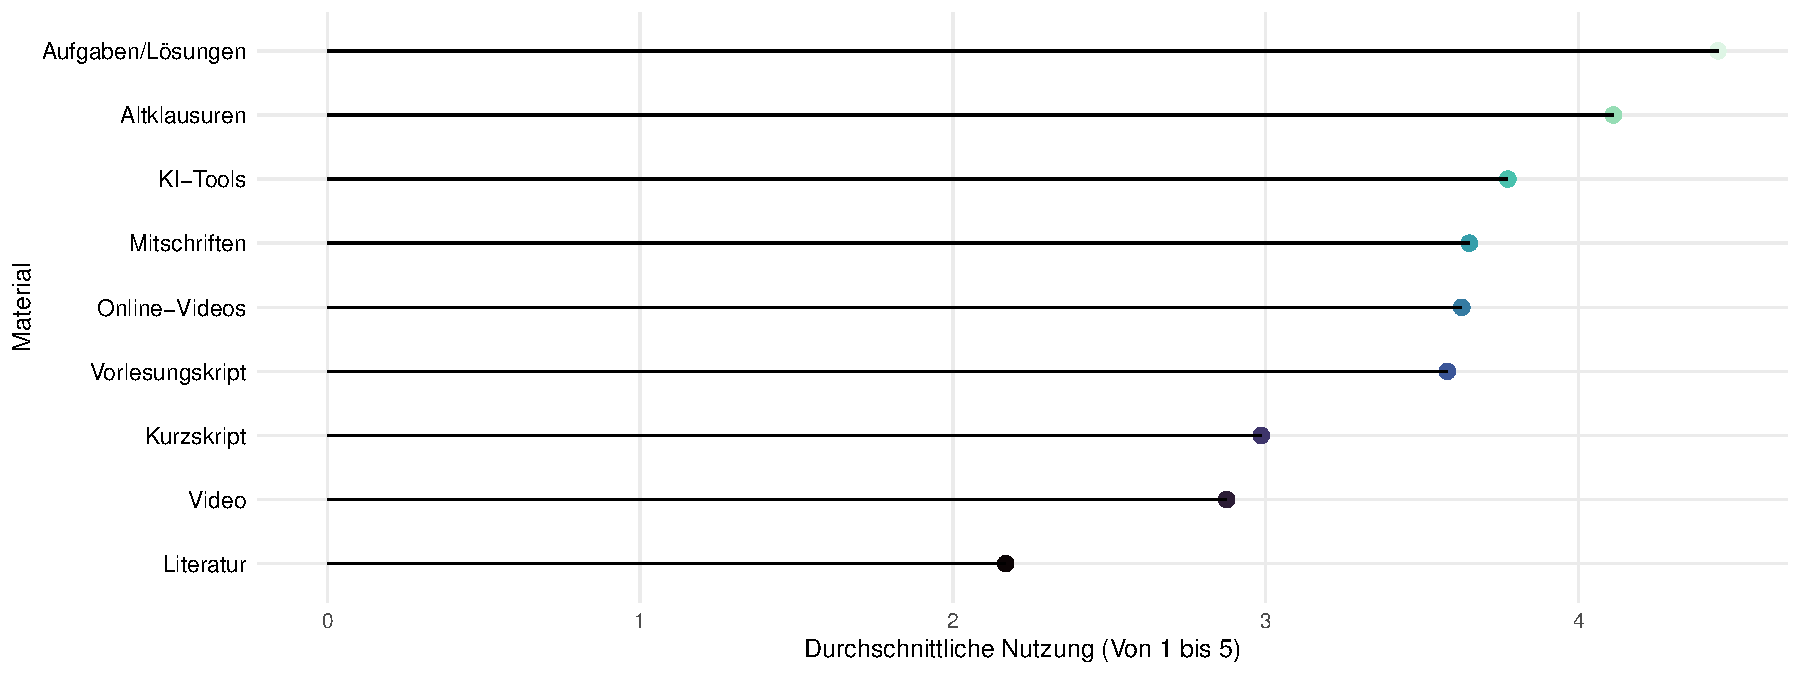
\includegraphics[width=0.9\textwidth]{Plot1.Nutzung.pdf}
    \caption{Durchschnittliche Nutzungshäufigkeit der Lernmaterialien (0-5) }
\end{figure}

Die Analyse der durchschnittlichen Nutzungshäufigkeit über alle Teilnehmenden hinweg zeigt deutliche Präferenzen der Studierenden. Es zeigt sich eine Dominanz prüfungsnaher, institutioneller Materialien mit Musterlösungen und Altklausuren, die mit Werten über $4{,}0$ am häufigsten genutzt werden. Bemerkenswert ist jedoch, dass auch digitale Hilfsmittel bereits im Lernalltag etabliert sind. YouTube und KI-Tools haben mit Nutzungswerten zwischen $3{,}5$ und $4$ eine Nutzungshäufigkeit, die vergleichbar ist mit der von klassischen Mitschriften. Sie weisen damit eine höhere Nutzungshäufigkeit auf als traditionelle Materialien wie das Kurzskript oder Vorlesungsvideos, welche sich im Mittelfeld bewegen (Werte bei ca. $3{,}0$). Am geringsten fällt die Nutzung klassischer Literatur aus, hier liegt der Durchschnittswert bei knapp über $2$, das am wenigsten genutzte erfasste Material. 
%Plot2%

\subsection{Korrelation der Materialien mit Zeitaufwand und Verständnis}

%Grafik Plot 2%
\begin{figure}[H]
    \centering
    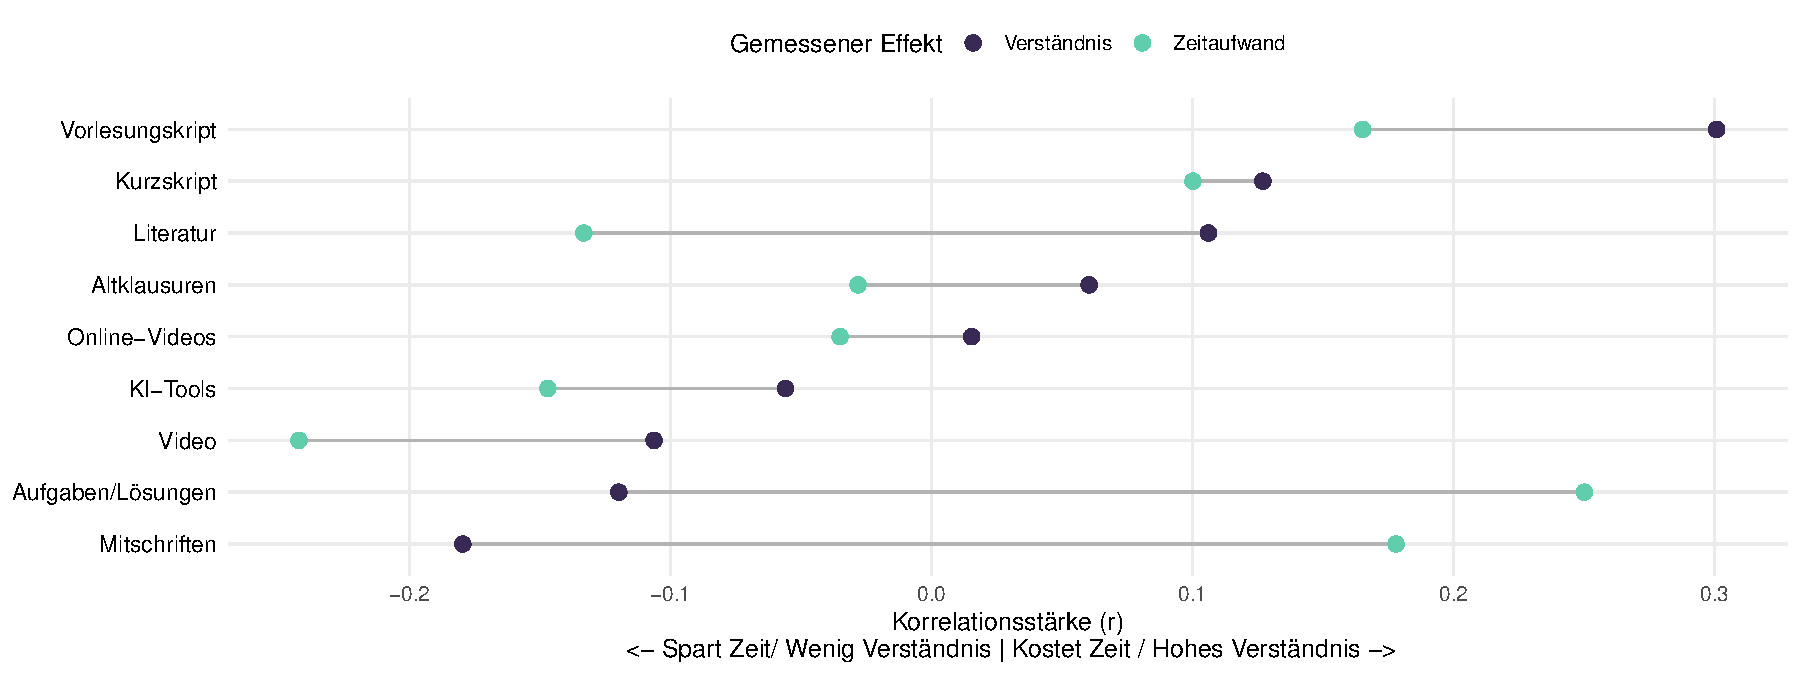
\includegraphics[width=0.9\textwidth]{Plot2.cor.time.verst.pdf}
    \caption{Korrelation von Lernmaterial mit subjektivem Zeitaufwand und Verständnis} 
\end{figure}
Betrachtet man die Ergebnisse in der Abbildung 2 fallen deutliche Zusammenhänge auf, das Vorlesungsskript korreliert am stärksten positiv mit dem Verständnis (Korrelationskoeffizient $0{,}3$) und hebt sich deutlich ab im Vergleich zu allen anderen Materialien. Allerdings auch im Bezug auf den Zeitaufwand, die Spanne zwischen Verständnis und Zeitkorrelation ist aber weiter als bei anderen Materialien, was darauf hindeutet, dass Skript eine höhere Zeiteffizienz als andere Materialien mit sich bringt, sowie zum Beispiel das Kurzskript. Das Kurzskript liegt zwar beim Verständnis auch vorn mit einer Korrelation bei etwa $0{,}12$, aber die Spanne zwischen der Korrelation des Zeitaufwandes und der Korrelation des Verständnisses liegt nahe beieinander, was darauf schließen lässt, dass im Verhältnis das Kurzskript weniger effektiv ist im Vergleich zu einem typischen Skript für den Lernerfolg. Am effizientesten jedoch finden sich die Bücher, deren Verständniskorrelation etwas geringer als die vom Kurzskript ist, aber der Zeitaufwand reiht sich eher mit dem von KI-Tools ein, was darauf deutet, dass das Lernen mit Büchern von Studierenden als sehr effizient empfunden wird. Altklausuren und YouTube ähneln sich im Zeitaufwand mit Korrelationswerten um die $-0{,}04$, allerdings ist das empfundene Verständnis bei Altklausuren etwas höher mit $0{,}06$ im Vergleich zu $0{,}01$. KI-Tools zeigen sich mit einem empfundenen Zeitaufwand von $0{,}15$ zwar als zeiteffizient, aber das Verständnis scheint dementsprechend auch im unteren Bereich der getesteten Optionen zu liegen. Die Verwendung von Vorlesungsaufzeichnungen korreliert am stärksten negativ mit dem empfundenen Zeitaufwand $< –0{,}2$, aber das empfundene Verständnis ist dafür auch am drittschlechtesten. Überraschend zeigen sich die Ergebnisse zu Musterlösungen und eigenen Mitschriften, welche im Vergleich zu allen anderen Materialien die größte Spanne zwischen Verständnis- und Zeitaufwandkorrelation haben, aber es sogar schaffen die Wirkungsrichtung des Graphen umzukehren, sodass das Verständnis hier negativ korreliert mit Werten zwischen $0{,}1$ und $0{,}2$ während der Zeitaufwand jedoch als höher empfunden wird mit Korrelationswerten zwischen $0{,}15$ und $0{,}3$. Zusammenfassend lässt sich feststellen, dass das Skript subjektiv als effektivste Lernmethode erscheint, während das Arbeiten mit Literatur als am effizientesten empfunden wird. 

\subsection{Verständnis nach Benutzergruppen}
%Grafik Plot 3%
\begin{figure}[H]
    \centering
    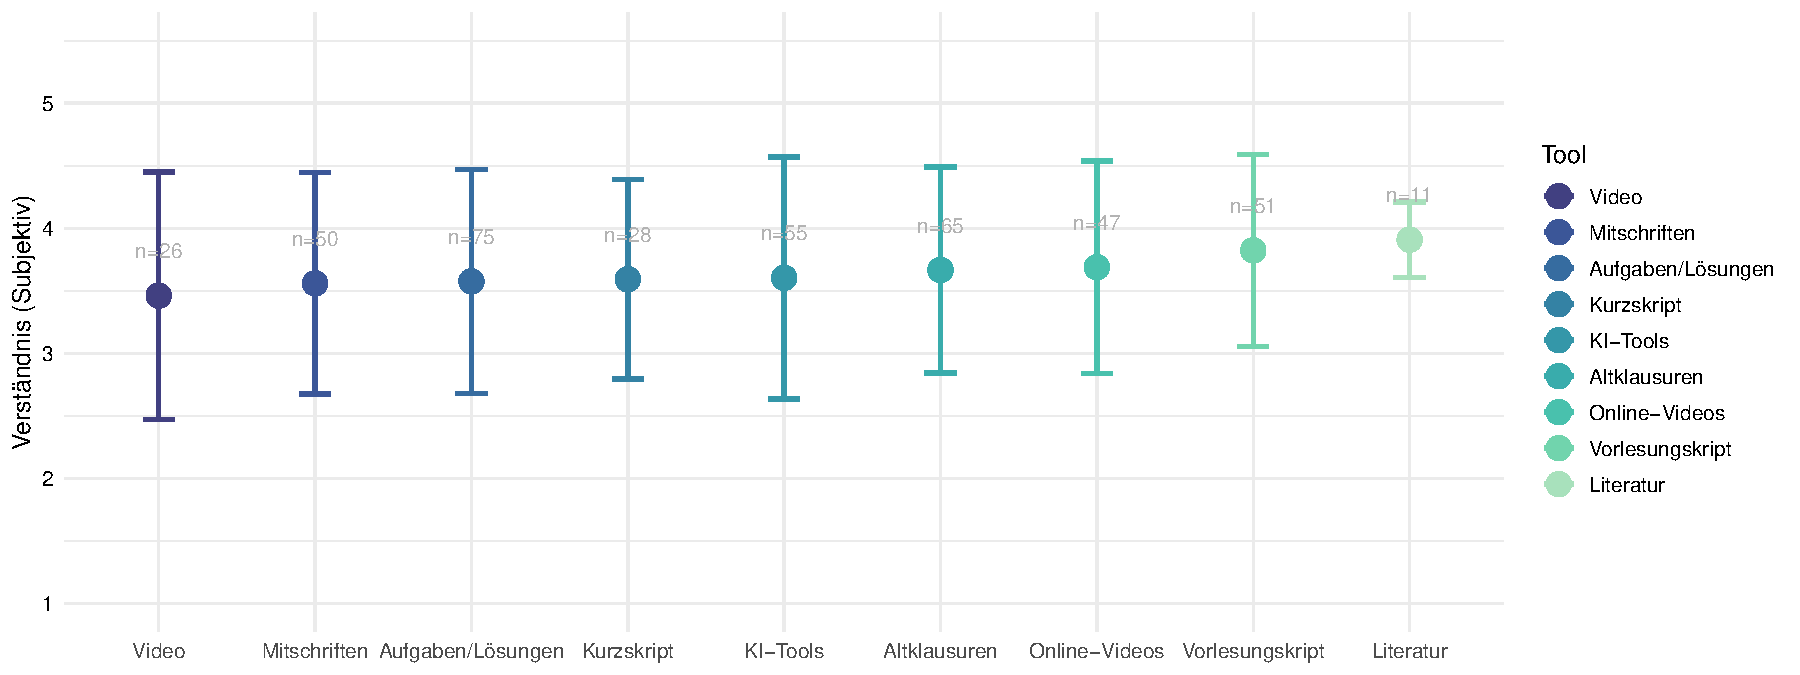
\includegraphics[width=0.9\textwidth]{Plot3.Errorplot.pdf}
    \caption{Empfundenes Verständnis bei Studierenden mit Intensivem Nutzungsverhalten} 
\end{figure}
Aus Abbildung 3 lassen sich einige Beobachtungen machen. Zwischen den beobachteten Gruppen zeigen sich hinsichtlich des durchschnittlichen Verständnisses nur geringe Unterschiede. Alle intensiven Nutzergruppen sind im durchschnittlichen Verständnis zwischen $3{,}4$ und $4{,}0$ zu finden. Jedoch lassen sich doch ein paar Besonderheiten zeigen. Bei den Intensivnutzern welche viel auf Bücher setzten ist die Streuung der Verständniswerte deutlich geringer als bei allen anderen Nutzergruppen während sie bei Studierenden welche KI-Tools benutzten am höchsten ist. Skript, YouTube und Altklausuren zeigen alle eine vergleichbare Streuung wie auch Nutzergruppengröße, welche im Verständnis im Durchschnitt leicht höher ist als bei Intensivnutzern von Kurzskript, Musterlösung und Mitschrift, jedoch eine vergleichbare Streuung aufweisen. Die Nutzergruppe mit einer intensiven Nutzung von Vorlesungsaufzeichnungen hat als einziges einen Wert $<3{,}5$ für das durchschnittliche Verständnis. Wichtig zu erwähnen ist das hier für Bücher mit einer kleinen Sichprobe garbeitet wird($n = 11$) weswegen man die Ergebnisse mit skepsis betrachten sollte.
\subsection{Verständnis Verteilung von Intensiven Nutzern}
%Grafik Plot 4%
\begin{figure}[H]
    \centering
    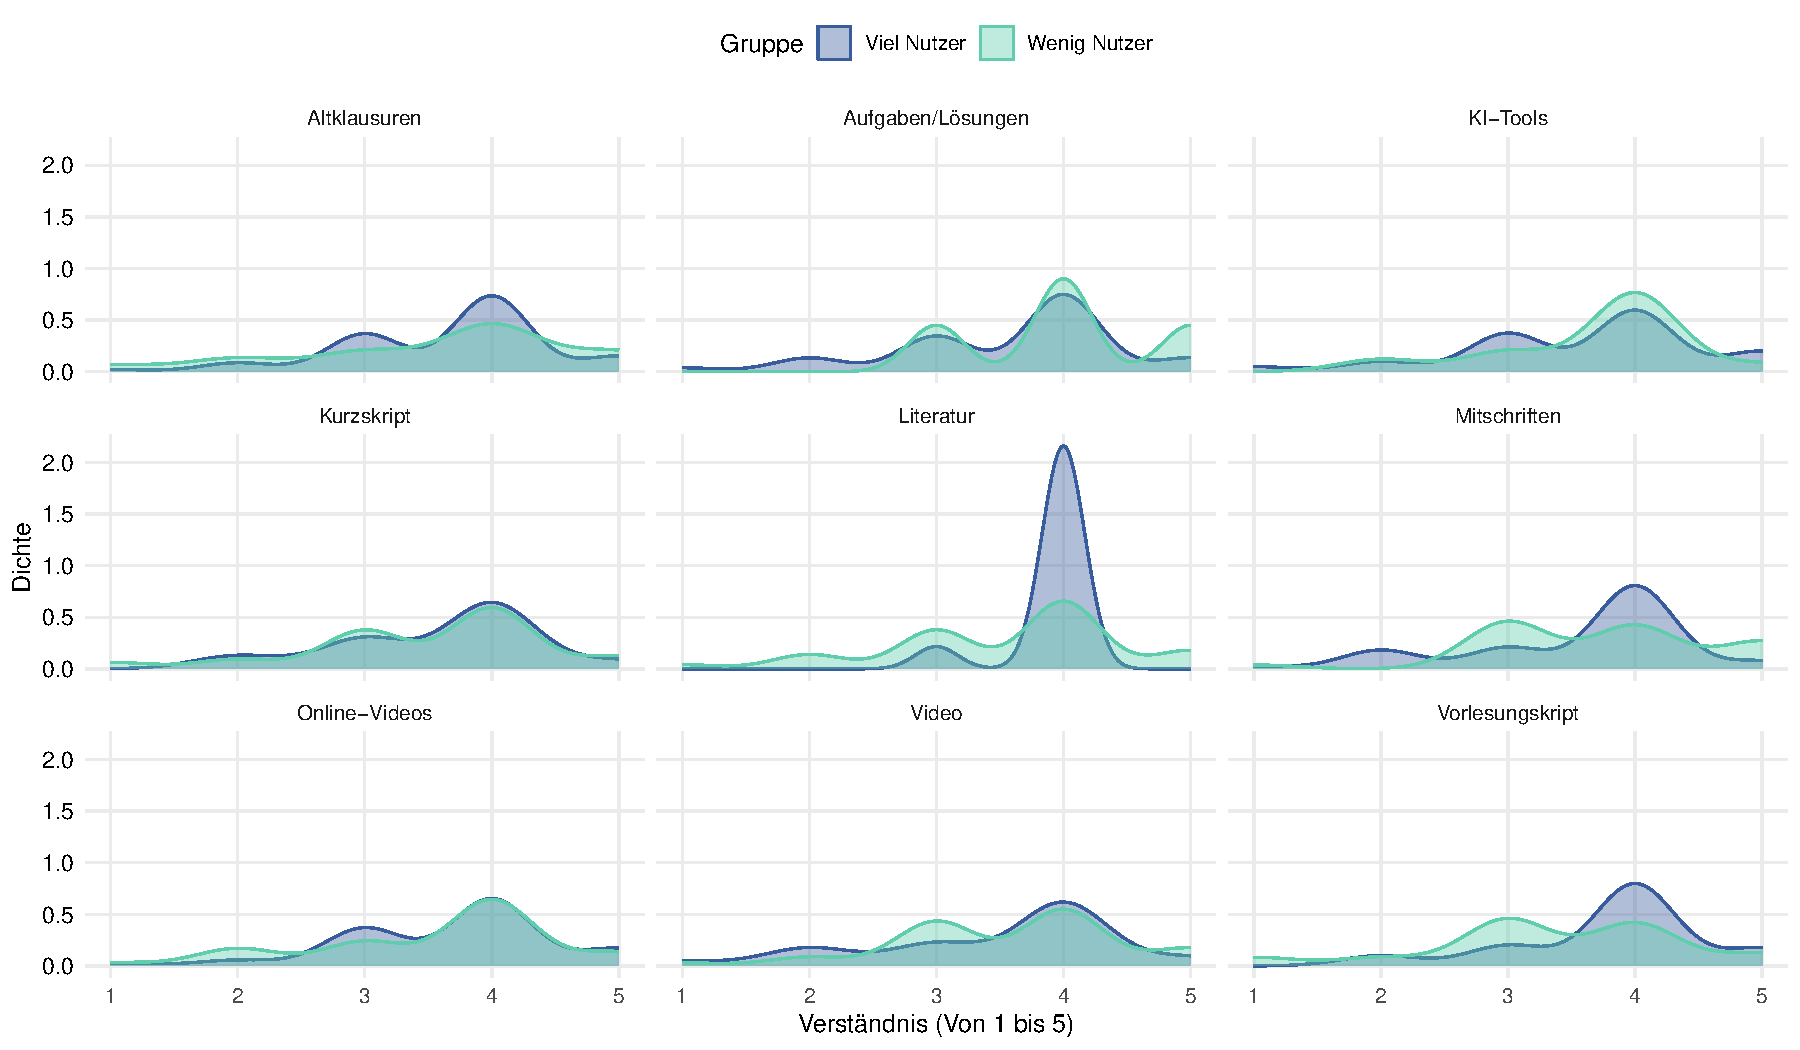
\includegraphics[width=0.9\textwidth]{Plot4.Verständnisdichte.pdf}
    \caption{Verteilung des Verständnis bei Intensiven Nutzern unterschiedlicher Materialien} 
\end{figure}
In der Abbildung 4 lassen sich einige Beobachtungen machen, die sich auch mit unseren restlichen Grafiken decken. Besonders fällt hier die Verständnisverteilung bei Menschen, die viele Bücher benutzen, auf, da diese sich zu großen Teilen in dem subjektiven Verständnis empfinden in der Bewertung um den Wert $4$ konzentriert, was im Vergleich zu anderen Intensivnutzern nur hier beobachtet werden kann. Die Wenignutzer des Skripts hingegen sind deutlich mehr gestreut, was die empfundene Zufriedenheit angeht, mit 3 lokalen Maxima, welche sich bei empfundenem Verständnis von $2$, $3$ und $4$ zeigen. Bei den Intensivnutzern des Skripts lässt sich auch eine leichte Diskrepanz finden: Intensivnutzer scheinen ein besseres empfundenes Verständnis zu haben als wenig Nutzer. Bei den digitalen Medien fallen die Ergebnisse anders aus. Hier zeigt sich sogar, dass die Verwendung von KI-Tools anscheinend das Verständnis eher leicht beeinträchtigt. Studierende, welche als Wenignutzer klassifiziert sind, schneiden subjektiv im Durchschnitt etwas höher ab als Studierende, die angeben, dass sie viel KI-Tools verwenden. Bei Intensivnutzern von YouTube läuft es ähnlich: Menschen, die nicht intensiv YouTube nutzen, scheiden  im Vergleich zu denen, die es  tun, fast identisch ab, es gibt einen leichten anstieg bei wenig Nutzern bei einem Verständnis von $2$ im Vergleich zu Vielnutzern, wo relativ gesehen ein paar mehr Studierende ein empfundenes Verständnis von $3$ angegeben haben. Außerdem lässt sich bei den Altklausuren feststellen das Intensivnutzer ein etwas höheres empfundenes Verständnis zeigen. Bei allen anderen Untersuchten Materialien sind die Effekte Minimal.
\subsection{Korrelation von Lerneffekten mit den Nutzungsmaterialien}
%Grafik Plot 4.5%
\begin{figure}[H]
    \centering
    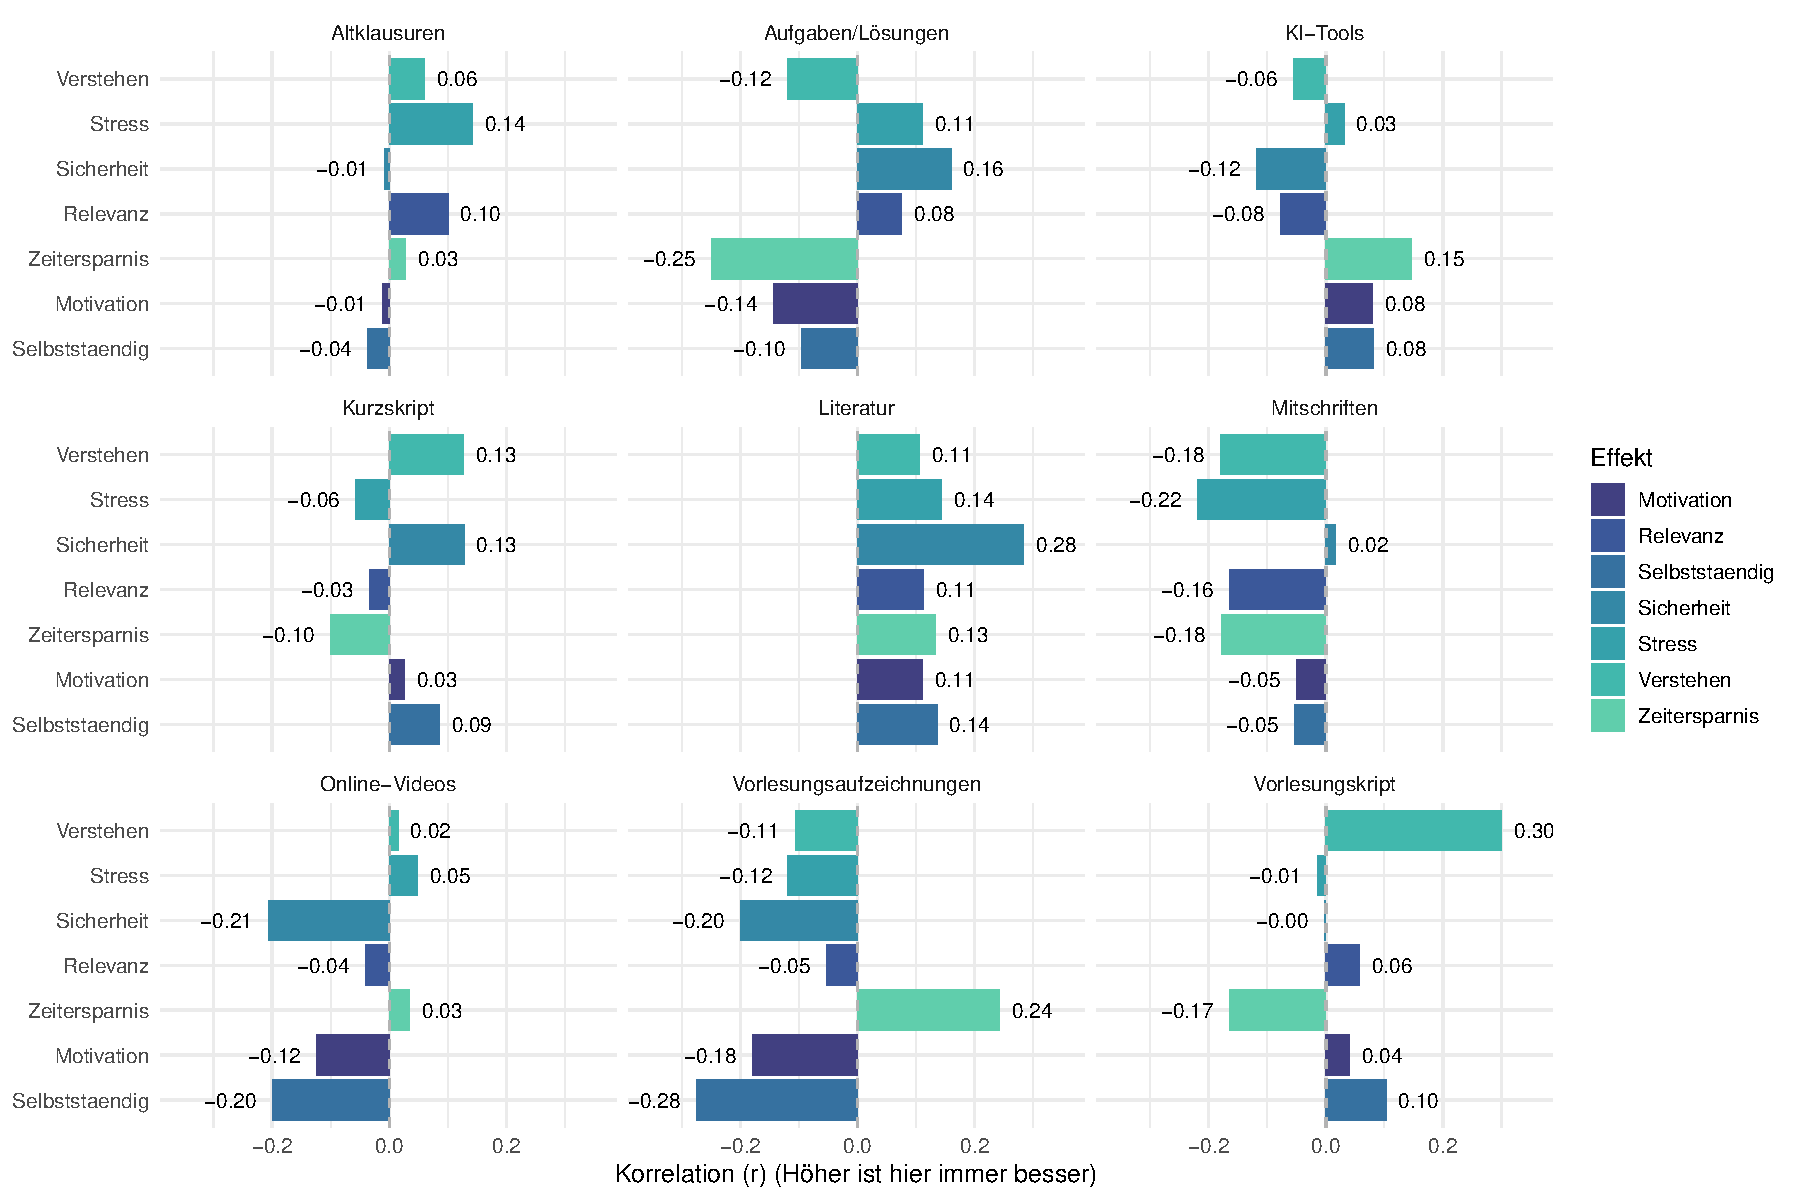
\includegraphics[width=0.9\textwidth]{Plot4.5.Korrelation.pdf}
    \caption{Welche Attribute korrelieren mit welchem Material} 
\end{figure}
In der Grafik lassen sich einige Zusammenhänge zeigen. Die Nutzung von Literatur zeigt durchgehend positive Korrelationen mit allen untersuchten vorteilhaften Attributen. Bis auf Altklausuren welche bis auf eine minimal negative Korrelation mit der Sicherheit sowie Motivation und Selbständigkeit auch leicht Positive Korrelationen mit allen anderen Attributen verzeichnen kann. Die digitalen Materialien KI und YouTube korrelieren beide leicht negativ mit der Sicherheit der Studierenden, während sie nur minimale positive Korrelationen mit Aspekten wie Stress oder Zeitaufwand zeigen können. Es zeigen sich allerdings leicht Positive Korrelationen ($r \ge 0.8$)  mit Motivation, Zeitersparnis sowie Selbstständigkeit bei dem verwenden von KI-Tools, welche aber bei der Verwendung von Online-Videos nicht im gleichen ausmaß zu sehen sind. Hier scheint die Selbständigkeit ($r = -0{,}2$) und Motivation ($r = -0{,}12$) leicht negativ zu Korrelieren. Bei den Mitschriften Korreliert alles außer die Sicherheit ($r = 0{,}02$) leicht negativ mit der Verwendung von Mitschriften. Auch Vorlesungsaufzeichnungen können bis auf eine Positive Korrelation mit der Zeitersparnis ($r = 0.24$) nur negative korrelationen mit allen anderen empfundenen Effekten verzeichnen
\subsection{Welche Attribute Korrelieren mit Zufriedenheit}
%Grafik Plot 5%
\begin{figure}[H]
    \centering
    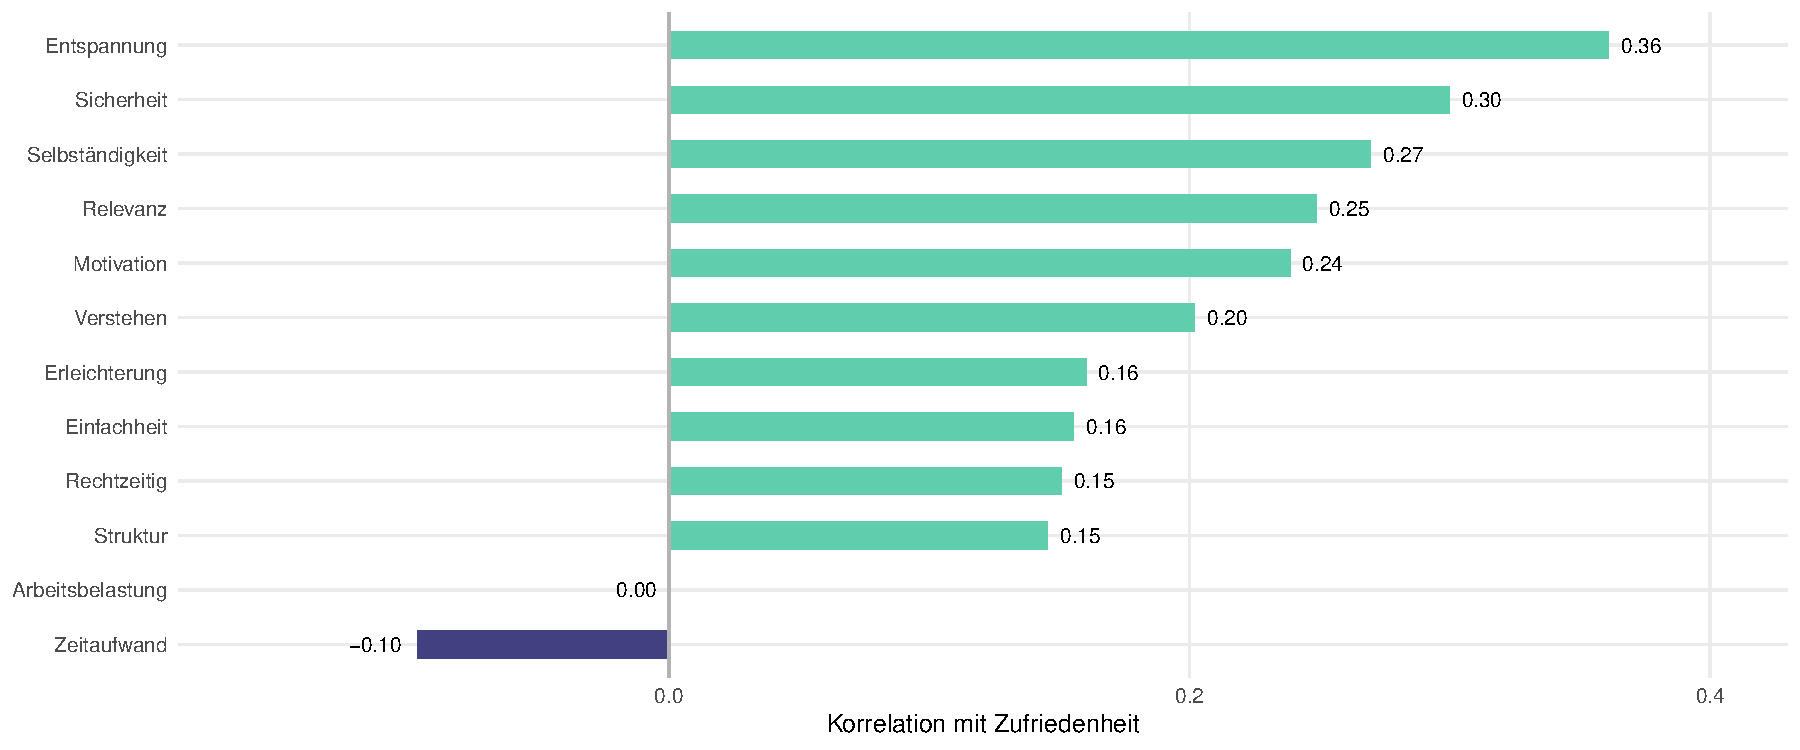
\includegraphics[width=0.9\textwidth]{Plot5.Effekt.cor.pdf}
    \caption{Wie Korrelieren Attribute mit Zufriedenheit} 
\end{figure}
Anhand der Abbildung lassen sich Einblicke in das tatsächliche Zufriedenheitsbild gewinnen: hier zeigt sich klar, dass Stress stark positiv mit der Zufriedenheit Korreliert gefolgt von Sicherheit, welche beide eine Positive Korrelation mit $\ge 0.3$ zeigen. Attribute wie Zeitaufwand sowie das Verständnis scheinen im Vergleich zu psychologischen Faktoren wie Stress oder Sicherheit eine untergeordnete Rolle für die Gesamtzufriedenheit zu spielen.
\subsection{Zwischenfazit zu den Ergebnissen}
Aus der deskriptiven Analyse der Daten lassen sich vier Kernbeobachtungen erkennen, welche als Grundlage für die Folgende Diskussion dienen: 
\begin{itemize}
    \item \textbf{Dominanz Institutioneller Materialien: } Institutionelle Materialien wie Musterlösungen und Altklausuren werden am Häufigsten verwendet. Allerdings haben YouTube als auch KI-Tools bereits Traditionelle Materialien wie Bücher oder Kurzskripte überholt. 
    \item \textbf{Diskrepanz zwischen Nutzung und Effektivität: } Materialien wie Musterloesungen und Mitschriften werden zwar viel genutzt, scheinen aber negativ mit Verständnis udn Zeiterstparnis zu korrelieren im Vergleich zu den meisten Untersuchten Materialien. 
    \item \textbf{Psychologische Faktoren im Vergleich zu Lerneffekten: } Die Gesamtzufriedenheit der Studierenden korreliert stärker mit psychologischen Faktoren wie stressreduktion und Sicherheit als mit direkten Einflussnehmern wie Zeitaufwand oder dem Verständnis. 
    \item \textbf{Digitale Tools und ihr Trugschluss: } KI-Tools sowie Youtube werden zwar als Zeiteffizient erlebt, korrelerien aber leicht negativ mit sowohl Sicherheit als auch dem Verständnis der Studierenden. 
\end{itemize}

% ==========================================
% 4. DISKUSSION
% ==========================================
\section{Diskussion}
Die Untersuchung zielte darauf ab, Zusammenhänge zwischen Lernmaterialien, deren Eigenschaften und der Zufriedenheit mit dem Lernerfolg aufzuzeigen. Hinsichtlich der ersten Forschungsfrage bestätigte sich die Annahme weitestgehend: Digitale Lernmaterialien sind aufgrund des geringen Zeitaufwands effizient, korrelieren jedoch kaum mit dem Verständnis. Vorlesungsvideos zeigen diesen Kontrast am deutlichsten, da sie den geringsten Zeitaufwand aufweisen, aber das drittschlechteste Verständnis. Dies deutet auf eine hohe Inhaltsdichte hin, die zwar Zeit spart, aber ein tiefes Verständnis erschwert, welches erst durch weitere Materialien gefestigt werden muss. Zusätzlich scheint die häufige Nutzung digitaler Materialien keinen signifikanten Einfluss auf das Verständnis zu haben. Grund dafür könnte eine Informationsflut durch die massive Fülle an verfügbaren Online-Inhalten sein, welche die kognitive Aufnahmefähigkeit schnell erschöpft. Zudem ist der geringe Zeitaufwand der einzige ersichtliche Vorteil digitaler Materialien, weswegen die Nachteile wie geringere Sicherheit, geringere Motivation und geringere Selbstständigkeit überwiegen. Bei den analogen bzw. institutionellen Materialien sticht das Skript besonders positiv hervor. Es weist die höchste Korrelation mit dem Verständnis (r = 0,3) und eine hohe Effizienz auf. Die Orientierung an der Vorlesung, wie auch die Kombination damit begünstigen hier vermutlich das Verständnis, wobei die Qualität und der Umfang vom Dozenten abhängt. Dies würde auch erklären, warum beim Kurzskript der Zeitaufwand tendenziell geringer und die Sicherheit höher ist. Bücher zeigten zwar die höchste Effizienz, durchgehend positive Korrelationen mit allen vorteilhaften Attributen und häufige Nutzung scheint sich sehr positiv auf das Verständnis auszuwirken, allerdings wurden sie durchschnittlich am wenigsten genutzt, weshalb die positiven Ergebnisse mit Skepsis zu betrachten sind. Gegenteilige Ergebnisse zeigten sich bei den Übungsaufgaben mit Musterlösungen. Obwohl sie am häufigsten genutzt werden, haben sie eine stark negative Effizienz und die zweitschlechteste Korrelation mit Verständnis. Vermutlich dienen sie eher der Vertiefung als dem inhaltlichen Neuerwerb, wofür gut strukturierte Skripte oder Bücher eher geeignet sind. Mitschriften schneiden ähnlich schlecht im Punkt Effizienz ab und gehen mit höherem Prüfungsstress, geringerem Verständnis und höherem Zeitaufwand einher. Übungsaufgaben mit Musterlösungen weisen dieselben Nachteile auf, aber hängen zumindest mit etwas weniger Stress und mehr Sicherheit zusammen. Insgesamt lässt sich bestätigen, dass während digitale Materialien mit Zeitersparnis punkten, analoge Materialien, mit Ausnahme von Musterlösungen und Mitschriften, ein höheres Verständnis fördern. Bezüglich der zweiten Forschungsfrage zum Zusammenhang zwischen Materialeigenschaften und der Zufriedenheit mit dem Lernerfolg ergab sich ein unerwartetes Bild. Entgegen der Annahme korreliert eher ein höherer Zeitaufwand mit dem subjektiven Lernerfolg (r = -0,1). Dieser kontraintuitiver Befund könnte damit zusammenhängen, dass sich zeitintensive Arbeit als wertvoller und produktiver empfunden wird. Das Verständnis spielt mit r = 0,2 ebenfalls eine geringere Rolle als erwartet. Ein Grund könnte sein, dass mit steigendem Wissen auch die Wahrnehmung eigener Wissenslücken zunimmt. Deutlich relevantere Faktoren für die Zufriedenheit mit dem Lernerfolg sind die psychologischen Wirkungseigenschaften, wie Reduktion von Prüfungsstress und Sicherheit, da diese am stärksten mit ihr korrelieren. Man könnte also behaupten, dass das psychische Wohlbefinden und die Emotionen im Zusammenhang mit dem Lernen, mehr Einfluss auf den subjektiven Lernerfolg haben, als zum Beispiel die Qualitätseigenschaften.Insgesamt lässt sich unsere zweite Annahme also nicht bestätigen, da sowohl Zeitaufwand als auch Verständnis nicht die ausschlaggebenden Faktoren bezüglich der Zufriedenheit mit dem Lernerfolg bilden. Limitationen: Die Zufriedenheit mit dem Lernerfolg korreliert nur gering mit den Einzelitem, was darauf hindeutet, dass sie von vielen individuellen Faktoren oder der Kombination verschiedener Materialien abhängt. Zudem erschwert die Repräsentation der Zufriedenheit mit dem Lernerfolg durch ein einziges Item die statistische Aussagekraft. Fazit: Die optimale Strategie für eine hohe Zufriedenheit mit dem Lernerfolg scheint in der primären Nutzung strukturierter, institutioneller Lernmaterialien zu liegen. Online-Videos oder KI-Chatbots können dabei zielgerichtet als Ergänzung genutzt werden, um die Effizienz zu steigern, ohne das tiefere Verständnis zu gefährden. Letztendlich hängt der subjektive Lernerfolg weniger von technischen Beschaffenheiten, sondern vielmehr von psychologischen Faktoren wie Prüfungsstress und Sicherheitsgefühl ab. Zukünftige Untersuchungen sollten daher vermehrt auf individuelle Lernstrategien und -fähigkeiten, psychologische Faktoren, sowie Langzeitstudien in den Fokus rücken.==========================================
% 5. REFLEXION
% ==========================================
\section{Reflexion}
Rückblickend lässt sich in der Konstruktion des Fragebogens sowie bei der Erhebung der Daten Verbesserungslücken erkennen, dessen Verbesserung die Validität und Ausagekraft der Ergebnisse erhöhen könnten. Ein zentraler Aspekt der Erhebung ist die „Zufriedenheit mit dem Lernerfolg“, welcher im Fragebogen zu Beginn platziert wurde, primär mit der Intention, einen „Aufmerksamkeits-Catcher“ zu generieren. Methodisch betrachtet wirft diese Positionierung allerdings ein Problem auf, da die Teilnehmer zu Beginn der Befragung möglicherweise aufgrund von unzureichender Reflexion über den momentanen Lernprozess ein zu voreilige Aussage treffen, was zu einer über- oder unterschätzten Selbsteinschätzung führen kann. Erst durch die Bearbeitung der darauffolgenden, spezifischeren Fragen findet eine tiefergehende Auseinandersetzung mit dem eigenen Lernverhalten statt, weswegen eine Platzierung am Ende des Fragebogens wahrscheinlich zu einer akkurateren Antwort geführt hätte. Zudem wurde das Merkmal „Zufriedenheit mit dem Lernerfolg“ lediglich durch ein einziges Item repräsentiert, obwohl es sich dabei um ein hochkomplexes, facettenreiches Empfinden handelt. Ein Single-Item reicht also nicht aus um die gesamte bandbreite dieses Merkmals abzudecken und zudem leidet darunter auch die Interpretation des Merkmals, da jeder Mensch „Zufriedenheit mit dem Lernerfolg“ unterschiedlich interpretiert und von unterschiedlichen Faktoren abhängig macht. Das erklärt vermutlich auch, warum die Zufriedenheit mit dem Lernerfolg kaum mit den erhobenen Materialeigenschaften korreliert. Bei einer erneuten Untersuchung müsste dieses Merkmal demgemäß durch eine Skala mit mehreren Items operationalisiert werden, um eine höhere Reliabilität zu erzielen. Ein weiteres methodisches Ziel war die Einteilung der Studierenden in Gruppen, beispielsweise nach Strukturiertheit oder der Qualität des Übungsbetriebs. Die Strukturiertheit sollte beispielsweise anhand der Items „Einstellung Pflicht Ball Num“ und „Einstellung Aufschieben Num“ festgemacht werden. In der Analyse der Daten stellte sichn jedoch heraus, dass diese Items nicht miteinander korrelieren, wodurch die geplante Clusterung der Probanden somit nicht statistisch haltbar war. Allgemein lässt sich feststellen, dass die Fragen zur persönlichen Einstellung zum Studium kaum einen Beitrag zur Beantwortung der letztendlichen Forschungsfragen geleistet haben. Im Sinne der Testökonomie wäre es rückblickend sinnvoller gewesen, diese ungenutzten Variablen zugunsten einer tiefgehenderen Abfrage der Zufriedenheit mit dem Lernerfolg zu streichen. Eine weitere geplante Clusterung war die, bezüglich der Qualitäts- und Wirkungseigenschaften der Materialien. Es sollte einen übergeordneten „Qualitäts-Score“, jedoch ergab die Datenanalyse, dass die Items zur Qualität untereinander zu gering korrelieren. Mit einem Cronbachs Alpha von < 0,7 wurde die notwendige interne Konsistenz für eine Skalenbildung verfehlt, weshalb der Score verworfen wurde. Dies deutet darauf hin, dass die Teilnehmer die Qualitätsaspekte der Materialien sehr differenziert und unabhängig voneinander wahrnehmen. Im Gegensatz zu den Qualitäts- Items zeigten die Wirkungs-Items eine starke Korrelation untereinander, was darauf hindeutet, dass psychologische Effekte deutlich homogener wahrgenommen werden als rein sachliche Qualitätsmerkmale. Zusammenfassend lässt sich sagen, dass das Instrumentarium in Bezug auf die Wirkungseigenschaften gut funktionierte, jedoch bei der Erfassung der objektiven Qualitätsmerkmale und der subjektiven Zufriedenheit mit dem Lernerfolg Verbesserungsvermögen aufweist. Eine stärkere Fokussierung auf psychologische und andere individuelle Faktoren, wie zum Beispiel das individuelle Nutzungsverhalten oder Persönlichkeitsmerkmale, würde die Untersuchung künftig präzisieren.
\end{document}